%%%%%%%%%%%%%%%%%%%%%%%%%%%%%%%%%%%%%%%%%%%%%%%%%%%%%%%%%%%%%%%%%%%%%%%%%%%
%% This file is part of the book
%%
%% Algorithmic Graph Theory
%% http://code.google.com/p/graph-theory-algorithms-book/
%%
%% Copyright (C) 2009--2011 Minh Van Nguyen <nguyenminh2@gmail.com>
%%
%% See the file COPYING for copying conditions.
%%%%%%%%%%%%%%%%%%%%%%%%%%%%%%%%%%%%%%%%%%%%%%%%%%%%%%%%%%%%%%%%%%%%%%%%%%%

\documentclass{article}

\usepackage{subfigure}
\usepackage{tikz}
\usetikzlibrary{external}
\usetikzlibrary{trees}
\tikzexternalize{sample-binomial-heaps}

\begin{document}

\begin{figure}
\subfigure[Binomial heap as a forest.]{
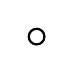
\begin{tikzpicture}
[-,thick,%
  every node/.style={shape=circle,inner sep=2pt,draw,thick},%
  scale=0.9]
\node {};
\end{tikzpicture}
%%
%%
\qquad
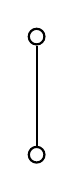
\begin{tikzpicture}
[-,thick,%
  every node/.style={shape=circle,inner sep=2pt,draw,thick}]
\node {}
  child {node {}};
\end{tikzpicture}
%%
%%
\qquad
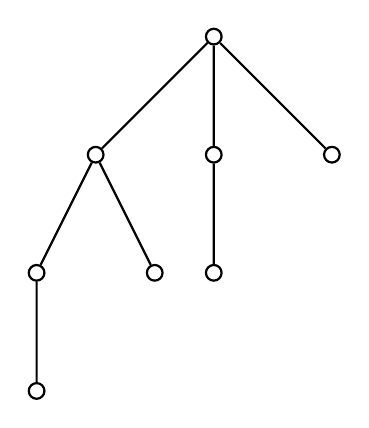
\begin{tikzpicture}
[-,thick,%
  every node/.style={shape=circle,inner sep=2pt,draw,thick}]
\node {}
  child {node {}
    child {node {}
      child {node {}}
    }
    child {node {}}
  }
  child {node {}
    child {node {}}
  }
  child {node {}};
\end{tikzpicture}
}
%%
%%
\qquad
\subfigure[Binomial heap as a tree.]{
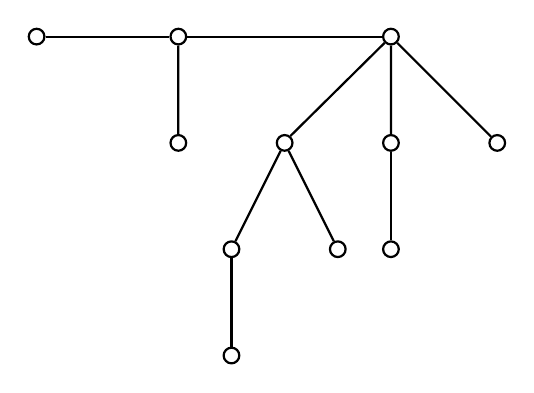
\begin{tikzpicture}
[-,thick,%
  every node/.style={shape=circle,inner sep=2pt,draw,thick},%
  scale=0.9]
\node (a) at (0,0) {};
%%
\node (b) at (2,0) {}
  child {node {}};
%%
\node (c) at (5,0) {}
  child {node {}
    child {node {}
      child {node {}}
    }
    child {node {}}
  }
  child {node {}
    child {node {}}
  }
  child {node {}};
\path
\foreach \startNode/\endNode in {a/b, b/c}
{
  (\startNode) edge[-,thick] (\endNode)
};
\end{tikzpicture}
}
\end{figure}

\end{document}
